\documentclass{article}
\usepackage{xeCJK}
\usepackage{listings}
\usepackage{minted}
\usepackage{graphicx}

\setsansfont{Ubuntu}
\setmonofont{Ubuntu Mono}
\setCJKmainfont{Noto Sans CJK SC}
\setCJKsansfont{Noto Sans CJK SC}
\setCJKmonofont{Noto Sans CJK SC}

\begin{document}
	\section{实验一\ 进程的建立}
		\subsection{实验目的}
			学会通过基本的 Windows 或者 Linux 进程控制函数,由父进程创建子进程,并实现父子进程协同工作。

		\subsection{实验软硬件环境}
			\texttt{Linux version 5.13.0-40-generic (buildd@ubuntu) \\ gcc (Ubuntu 9.4.0-1ubuntu1~20.04.1) 9.4.0,GNU ld (GNU Binutils for Ubuntu) 2.34}

		\subsection{实验内容}
			创建两个进程,让子进程读取一个文件,父进程等待子进程读取完文件后继续执行,实现进程协同工作。进程协同工作就是协调好两个进程,使之安排好先后次序并以此执行,可以用等待函数来实现这一点。当需要等待子进程运行结束时,可在父进程中调用等待函数。

		\subsection{实验程序及分析}
			\inputminted[linenos,breaklines,tabsize=4]{c}{lib1/lib1.c}

			使用 \mintinline{c}{fork()} 函数创建子进程。

			若 \mintinline{c}{fork()} 函数返回值等于 \texttt{0},则说明此进程为子进程。子进程读取文件并输出到屏幕,然后退出。

			若 \mintinline{c}{fork()} 函数返回值大于 \texttt{0},则说明此进程为父进程,返回值为子进程 PID。父进程中使用 \mintinline{c}{waitpid()} 函数挂起,等待子进程运行结束。

		\subsection{实验截图}
			\begin{figure}[htbp]
				\centering
				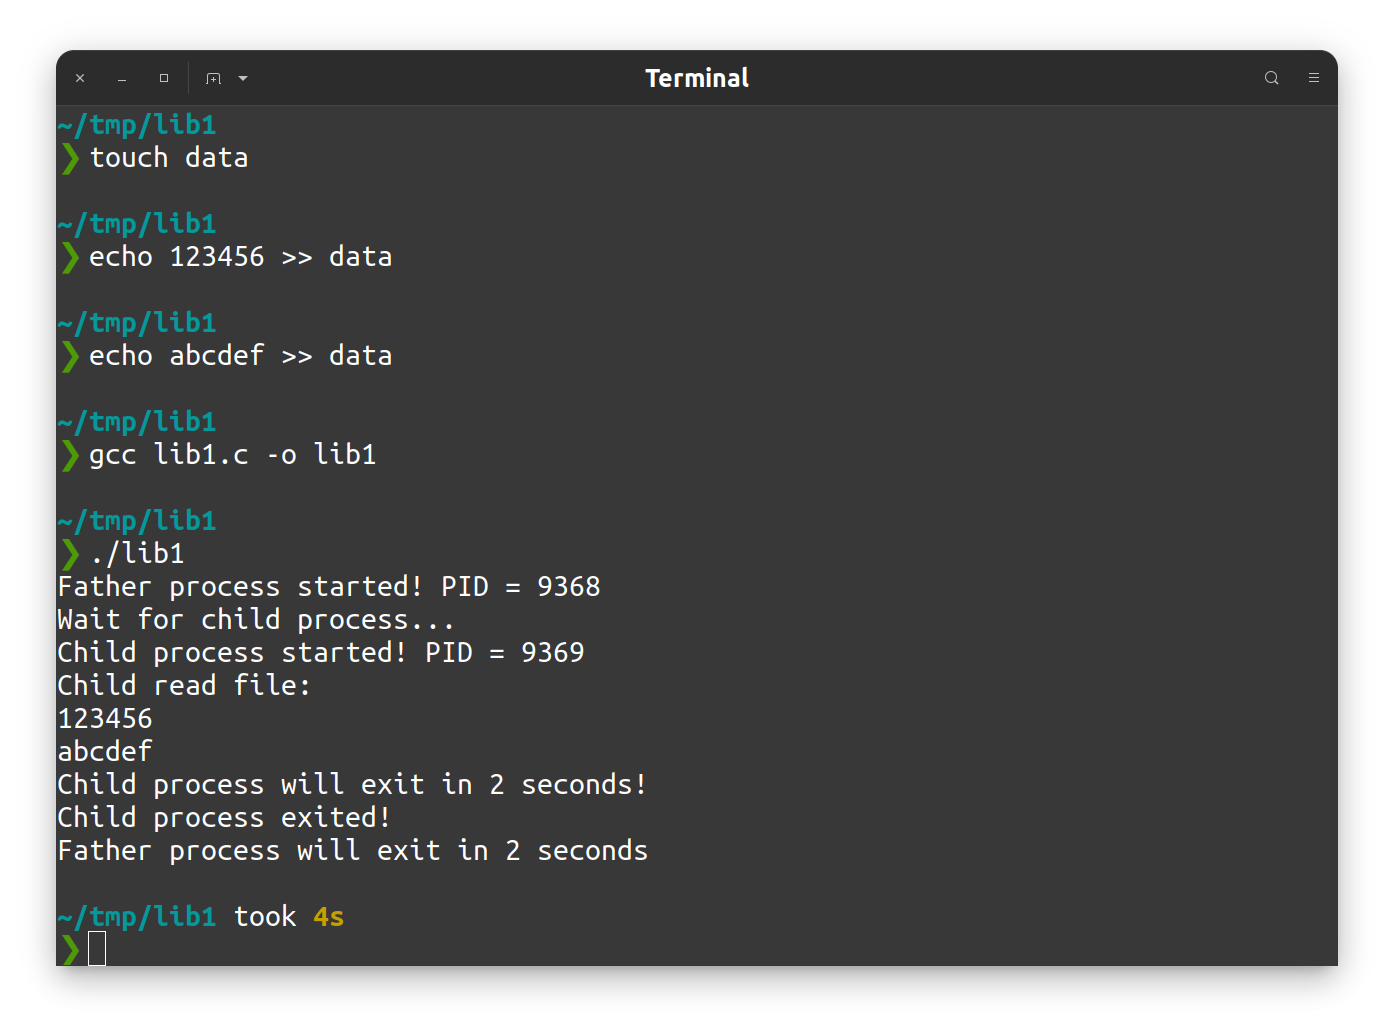
\includegraphics[width=\textwidth]{lib1/Screenshot.png}
				\caption{实验一\ 进程的建立}
			\end{figure}

		\subsection{实验心得体会}
			本次实验使用了 \mintinline{c}{fork()} 函数创建子进程,使用了 \mintinline{c}{waitpid()} 函数挂起父进程,达到父子进程协同工作的目的。通过实验,理解了进程的创建过程。

	\section{实验二\ 线程共享进程数据}
		\subsection{实验目的}
			了解线程与进程之间的数据共享关系。创建一个线程,在线程中更改进程中的数据。

		\subsection{实验软硬件环境}
			\texttt{Linux version 5.13.0-40-generic (buildd@ubuntu) \\ gcc (Ubuntu 9.4.0-1ubuntu1~20.04.1) 9.4.0,GNU ld (GNU Binutils for Ubuntu) 2.34}

		\subsection{实验内容}
			在进程中定义全局共享数据,在线程中直接引用该数据进行更改并输出该数据。

		\subsection{实验程序及分析}
			\inputminted[linenos,breaklines,tabsize=4]{c}{lib2/lib2.c}

			全局变量被进程和其子线程共享。故全局变量可被线程直接修改。

			使用 \mintinline{c}{pthread_create()} 函数创建线程。其中第三个参数是函数指针,表示线程执行函数。

			在进程中初始化全局共享变量并输出,然后在线程中修改全局共享变量并输出,最后等待线程函数执行完毕后,在进程输出全局共享变量。可以观察到线程成功修改了全局共享变量。

		\subsection{实验截图}
			\begin{figure}[htbp]
				\centering
				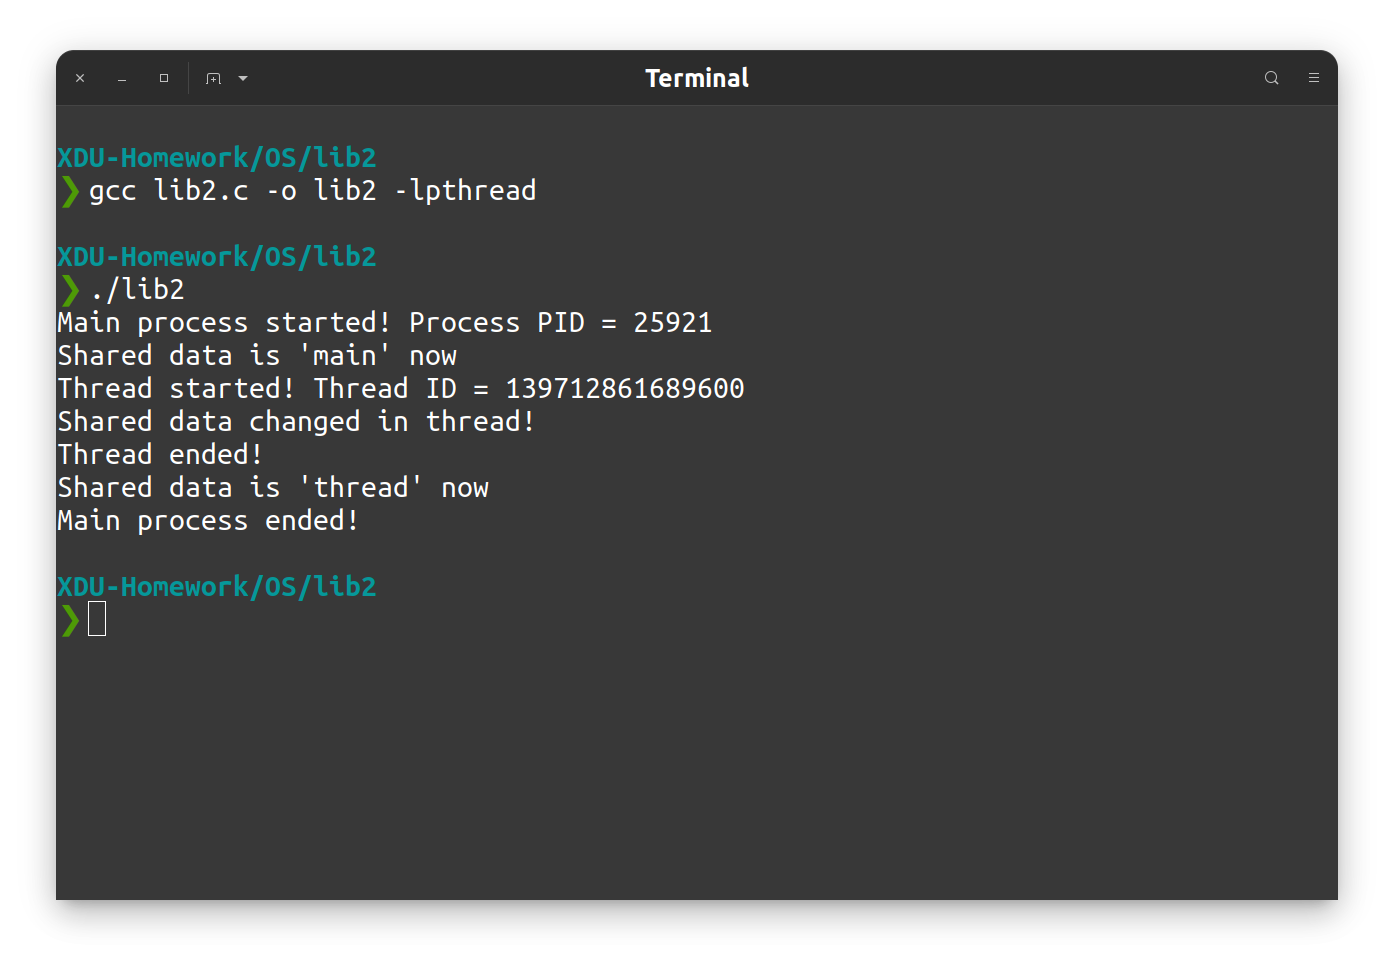
\includegraphics[width=\textwidth]{lib2/Screenshot.png}
				\caption{实验二\ 线程共享进程数据}
			\end{figure}

		\subsection{实验心得体会}
			本次实验使用了 \mintinline{c}{pthread_create()} 函数创建线程。并通过定义全局变量在进程和各个线程中共享,以达到线程通信的目的。通过本次实验,理解了如何定义全局共享变量,如何实现进程与线程之间的简单通信。

	\section{实验三\ 信号通信}
		\subsection{实验目的}
			利用信号通信机制在父子进程及兄弟进程间进行通信。

		\subsection{实验软硬件环境}
			\texttt{Linux version 5.13.0-40-generic (buildd@ubuntu) \\ gcc (Ubuntu 9.4.0-1ubuntu1~20.04.1) 9.4.0,GNU ld (GNU Binutils for Ubuntu) 2.34}

		\subsection{实验内容}
			父进程创建一个有名事件,由子进程发送事件信号,父进程获取事件信号后进行相应的处理。

		\subsection{实验程序及分析}
			\paragraph*{阻塞型通信}
				\inputminted[linenos,breaklines,tabsize=4]{c}{lib3/lib3_1.c}

				一个进程终止或者停止时,SIGCHILD 信号将被发送给其父进程。

				创建一个子进程,打印子进程 PID。子进程运行一段时间后退出。

				父进程调用信号处理函数 \mintinline{c}{signal()}, 捕获信号 SIGCHLD 并在 \mintinline{c}{handler()} 函数中处理。在 \mintinline{c}{handler()} 函数中输出退出的子进程的 PID。可以观察到,父进程成功捕获子进程的终止信号。

			\paragraph*{非阻塞型通信}
				\inputminted[linenos,breaklines,tabsize=4]{c}{lib3/lib3_2.c}

				在 Terminal 中按 \texttt{Ctrl + C} 可发送中断信号 SIGINT。

				父进程调用信号处理函数 \mintinline{c}{signal()}, 捕获信号 SIGINT 并在 \mintinline{c}{handler()} 函数中打印信息。

		\subsection{实验截图}
			\begin{figure}[htbp]
				\centering
				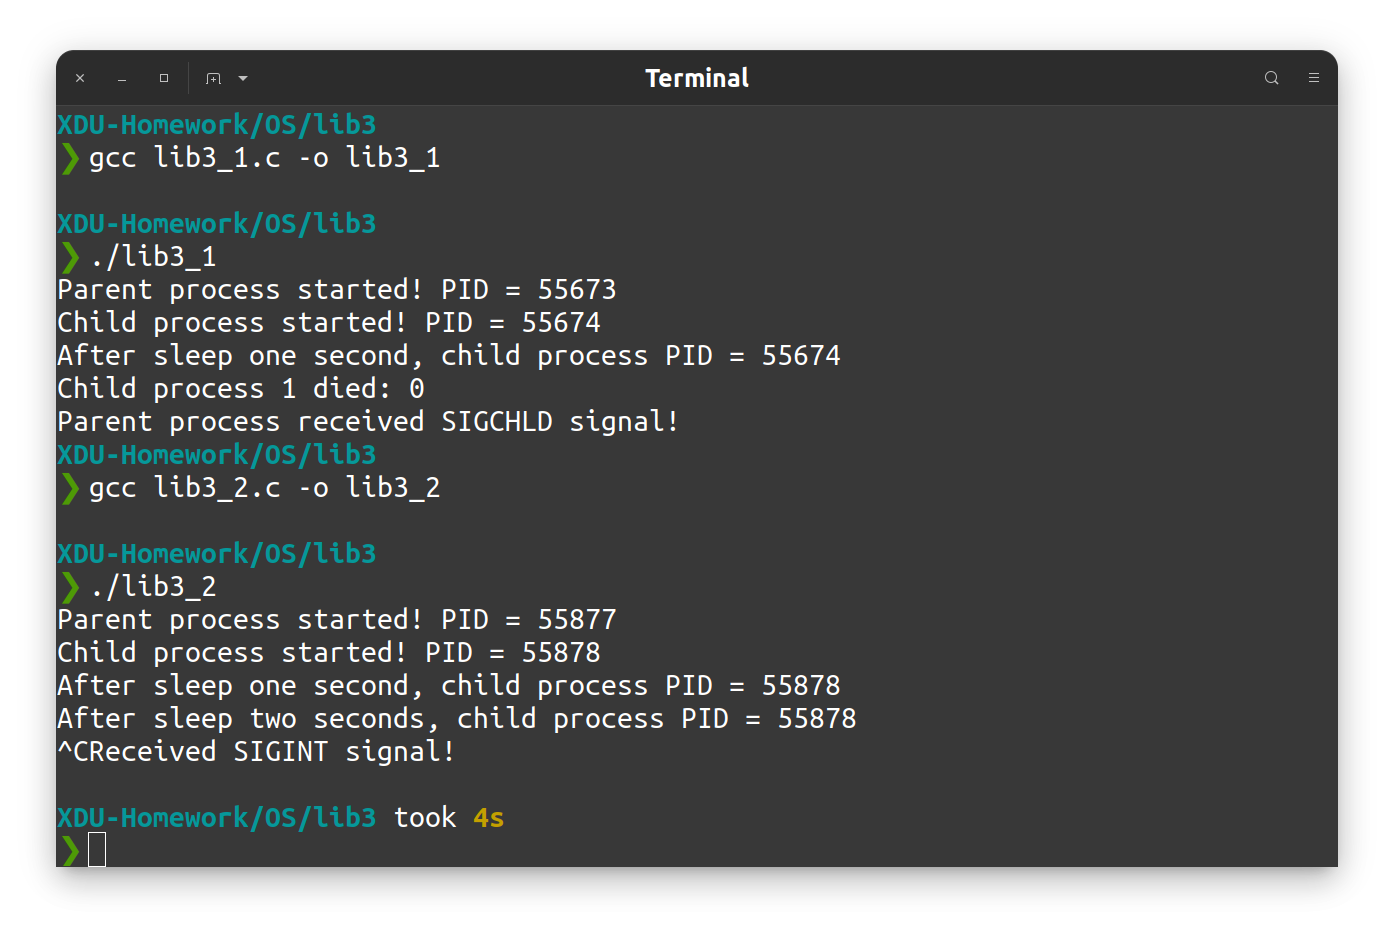
\includegraphics[width=\textwidth]{lib3/Screenshot.png}
				\caption{实验三\ 信号通信}
			\end{figure}

		\subsection{实验心得体会}
			本次实验使用了 \mintinline{c}{signal()} 函数捕获信号并做相应的处理。通过本次实验,理解了如何在进程之间进行信号通信。

\end{document}


